\documentclass[english, DIV=13]{scrartcl}

% Packages
\usepackage{pgfplots}
\usepackage{amsmath,amsfonts,amssymb}
\usepackage{empheq}
\usepackage{hyperref}
\usepackage{todonotes}

\renewcommand{\vec}[1]{\mathbf{#1}}

\title{LINMA1731 - Project}
\author{Antoine Paris\and Matthieu Xhonneux}
\date{\today}

\begin{document}
\maketitle

\section{Discrete-time version of the Lorenz system}
The Lorenz dynamical system is given by
\begin{equation*}
    \begin{cases}
        \dot{x} &= a(y-x) \\
        \dot{y} &= x(r-z) \\
        \dot{z} &= xy - bz
    \end{cases}.
\end{equation*}
Using first-order forward finite difference, that is approximating $\dot{x}(t)$ by
\[ \frac{x(t+\delta t) - x(t)}{\delta t} := \frac{x_{k+1} - x_k}{\delta t}, \]
a discrete-time version of the form
\[ \vec{x}_{k+1} = F(\vec{x}_k) + \Gamma\vec{u}_k \]
can be obtained. In this case, the function $F$ is given by
\begin{equation*}
    \begin{cases}
        F_1(\vec{x}_k) &= ay_k\delta t + (1-a\delta t)x_k \\
        F_2(\vec{x}_k) &= x_k(r-z_k)\delta t + (1-\delta t)y_k \\
        F_3(\vec{x}_k) &= x_ky_k\delta t + (1-b\delta t)z_k
    \end{cases}.
\end{equation*}

\section{3D-system simulation and noisy measurements}
A sample trajectory resulting from a 50 seconds simulation is given in figure~
\ref{fig:q2-3d-trajectory}. As expected for this set of paramaters, the trajectory
is chaotic and shows the typical ``figure eigth'' form. 

\begin{figure}[ht!]
    \centering
    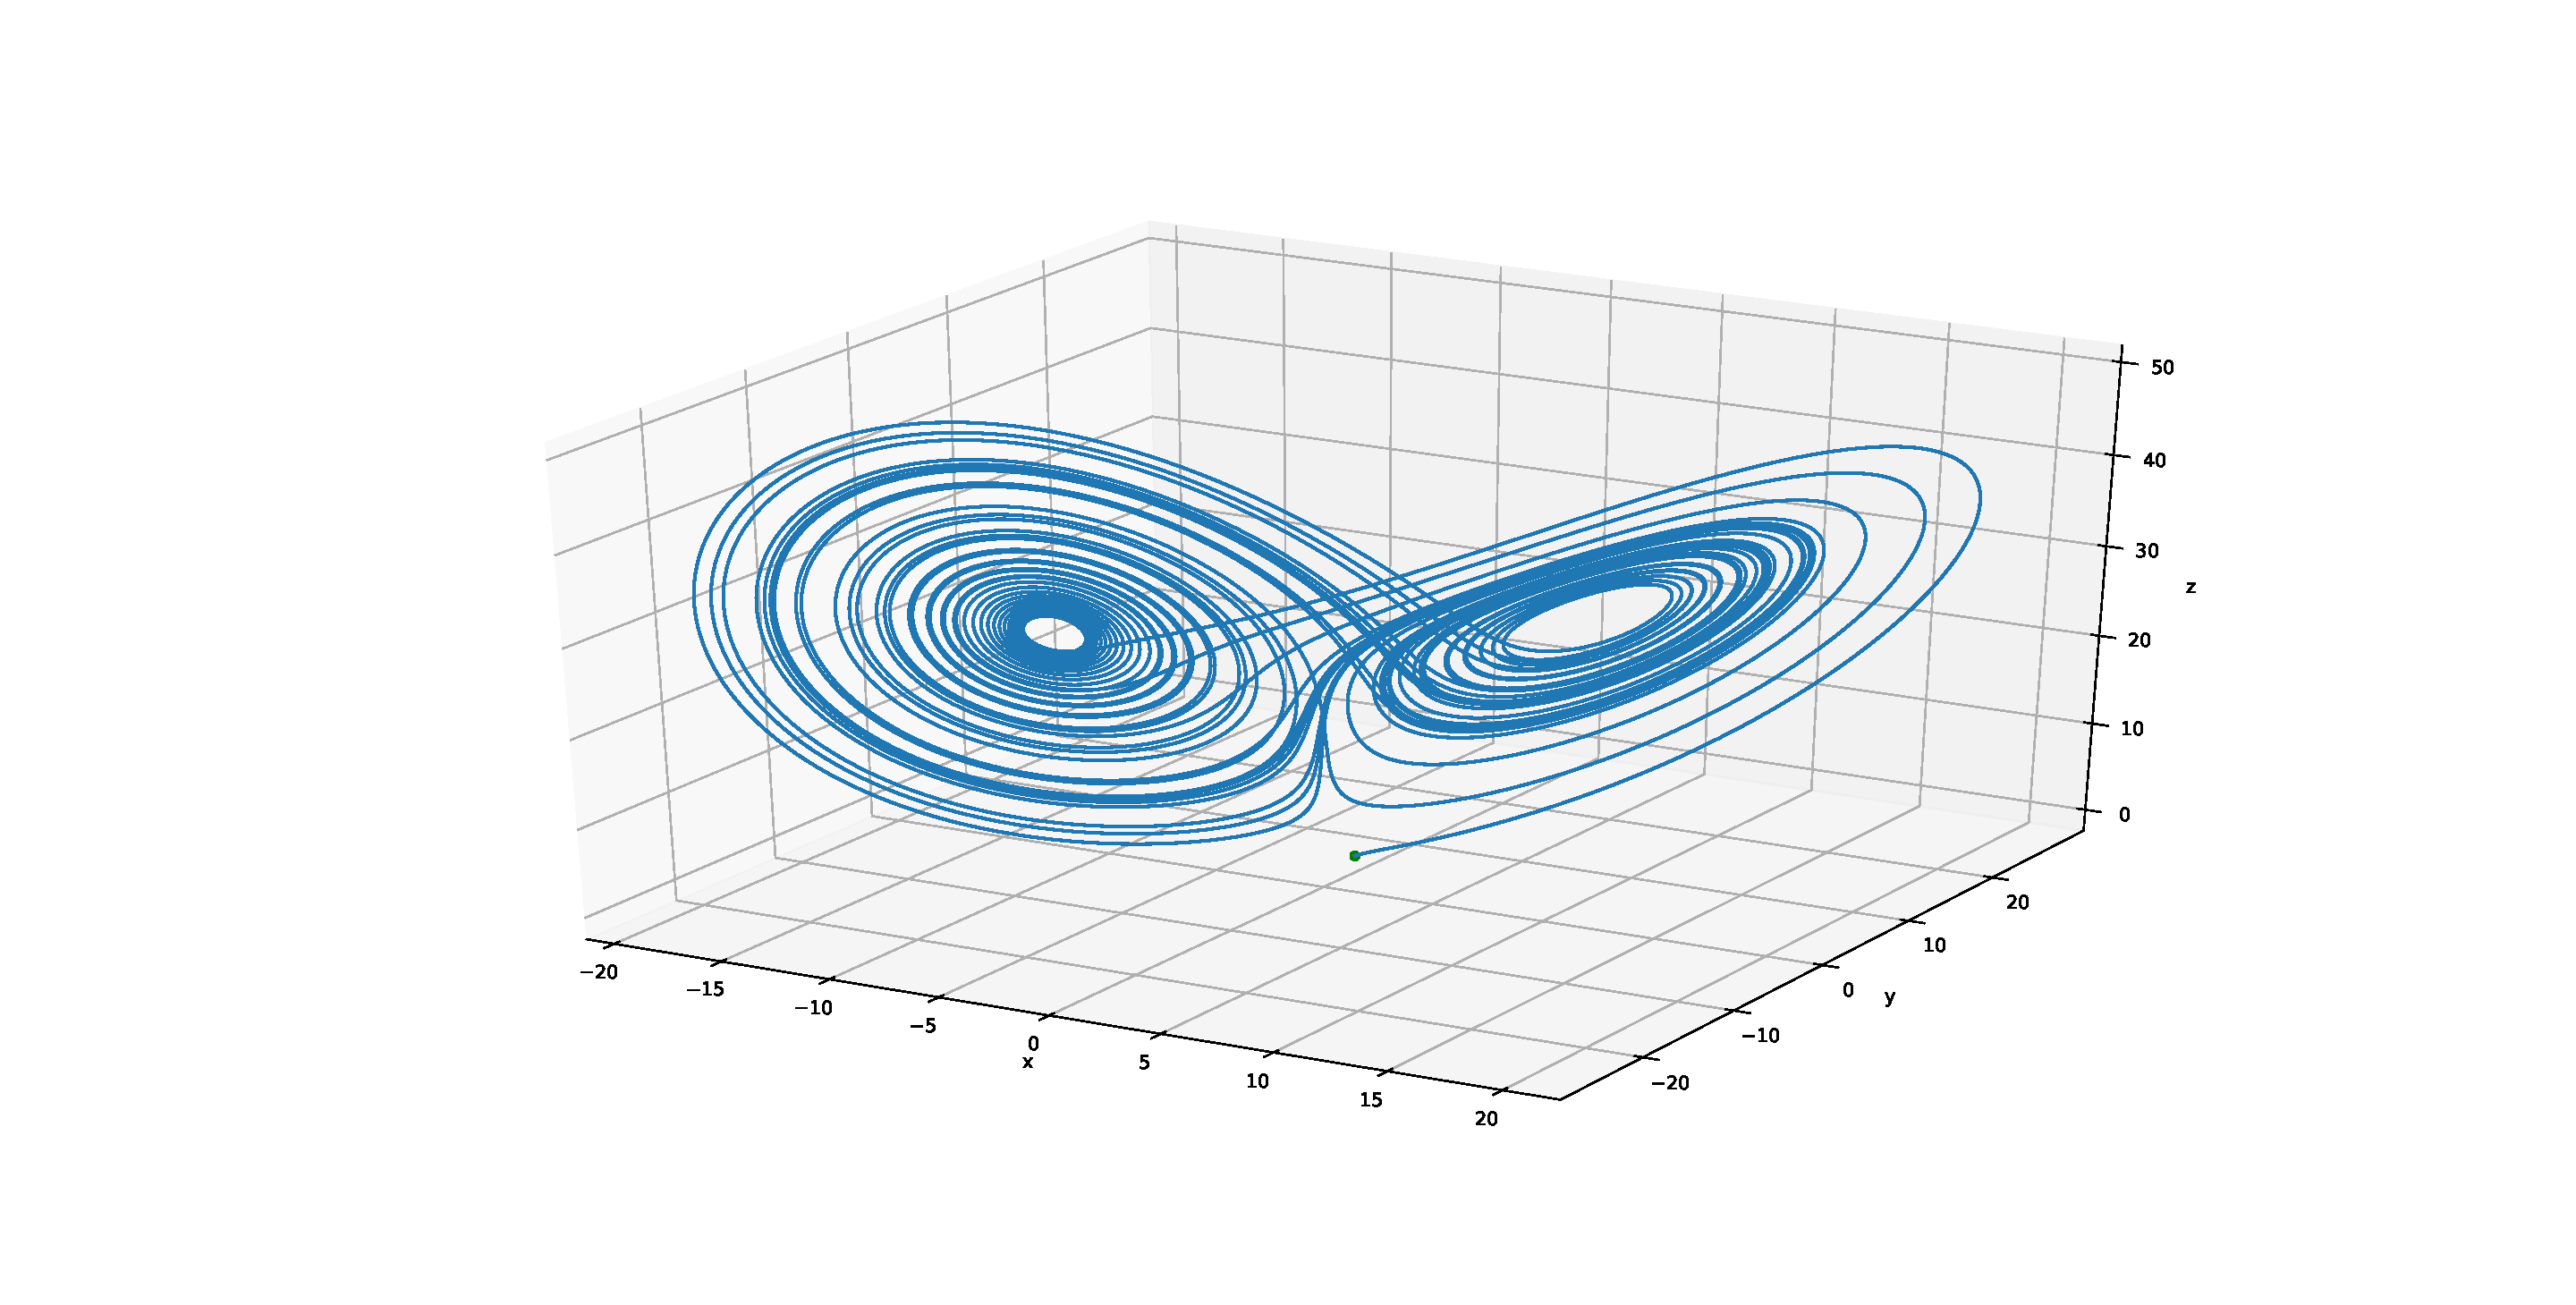
\includegraphics[width=0.75\textwidth]{figures/q2-3d-trajectory}
    \caption{Realization of a 50 seconds simulated trajectory. The initial
    position is indicated by the green dot. The resulting trajectory is chaotic
    (as expected for this set of paramaters).}
    \label{fig:q2-3d-trajectory}
\end{figure}

The trajectory of the first coordinates and the corresponding noisy measurements
are represented in figure~\ref{fig:q2-mes-vs-real}.

\begin{figure}[ht!]
    \centering
    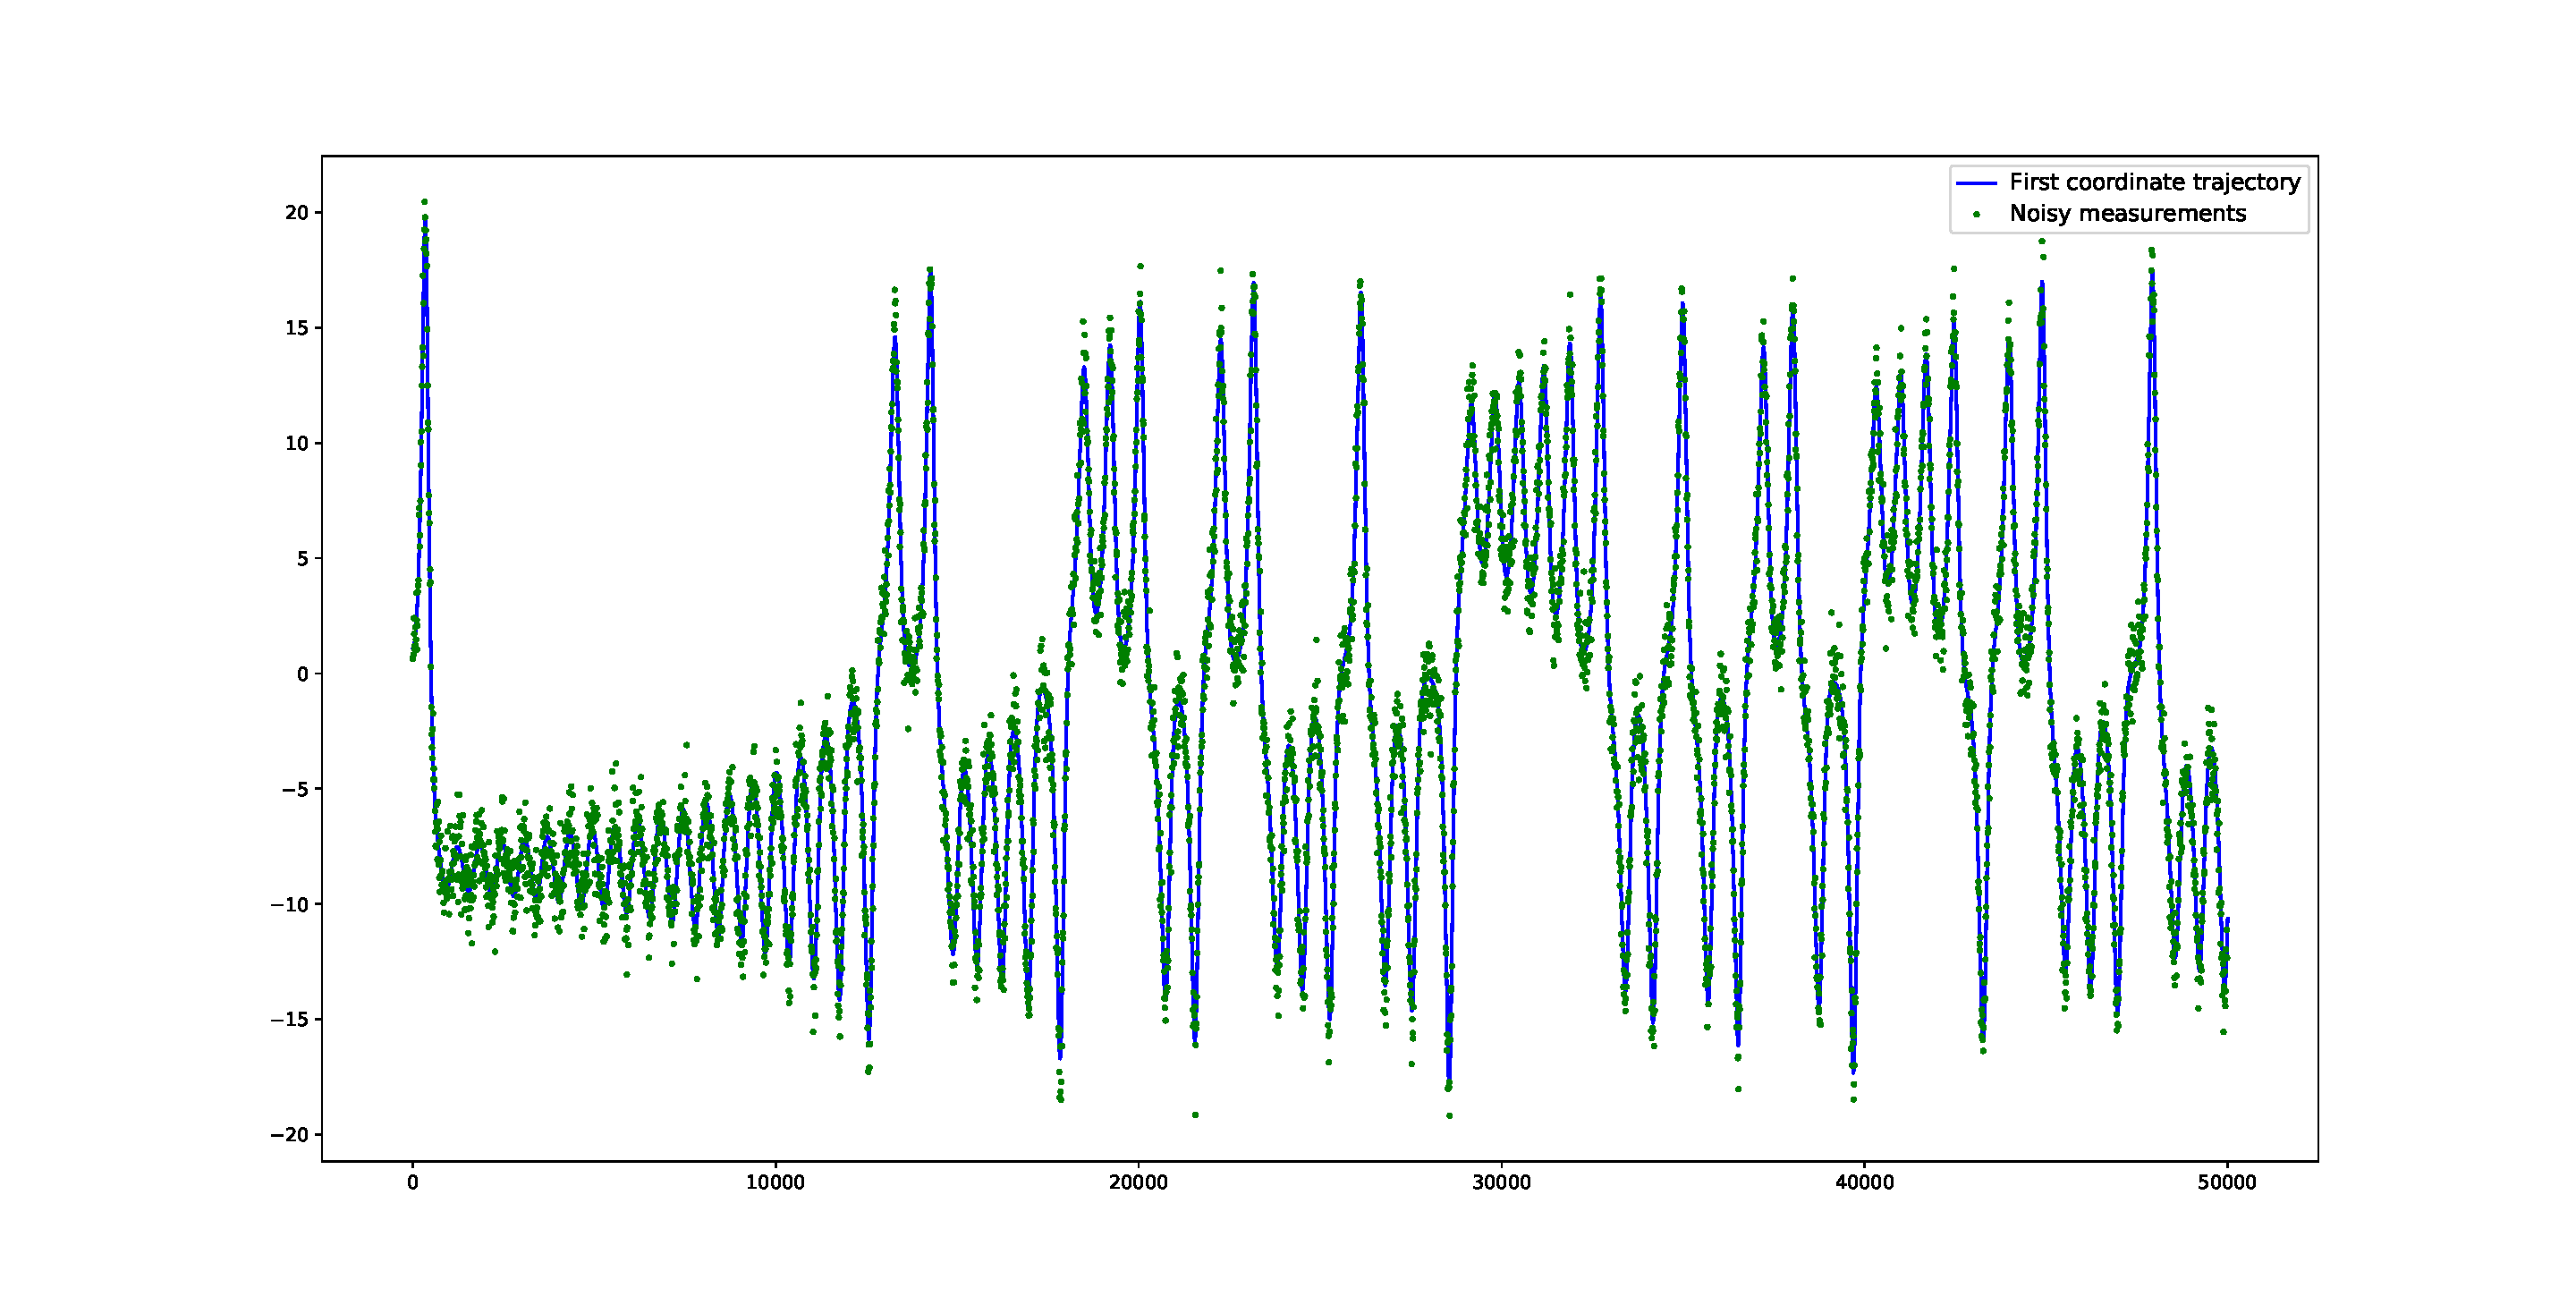
\includegraphics[width=0.75\textwidth]{figures/q2-mes-vs-real}
    \caption{Trajectory of the first coordinates and corresponding noisy measurements.}
    \label{fig:q2-mes-vs-real}
\end{figure}


\section{Implementation of an Extended Kalman Filter}

The Extended Kalman Filter amounts to applying a regular Kalman filter to the linearization of the system. Our system can be represented as :


\begin{equation*}
    \begin{cases}
        \vec{x}_{k+1} = F(\vec{x}_k) + \Gamma\vec{u}_k \\
        m_k = x_k + w_k
    \end{cases}.
\end{equation*}

In order to linearize this system, we need to compute the jacobian of $F$, for each time step $k$ :

\begin{equation*}
F_k = 
    \begin{pmatrix}
        1 - a \delta t & a \delta t & 0 \\
        (r - z_k) \delta t & 1 - \delta t & - x_k \delta t \\
        y_k \delta t & x_k \delta t & 1 - b \delta t
    \end{pmatrix}
\end{equation*}

We can then directly apply the Kalman Filter's equations. For prediction :


\[ \vec{\hat{x}}_{k|k-1} = F(\vec{x}_{k-1|k-1}) \]
\[ \vec{P}_{k|k-1} = \vec{F}_{k-1} \vec{P}_{k-1|k-1} \vec{F}_{k-1}^\mathsf{T} + \vec{Q} \]

with $\vec{Q} = \vec{\Gamma} \sigma_u^2$ the covariance matrix of the dynamics' noise.\\
For the update, we can't directly compute the Kalman gain like this :

\[ \vec{K}_k = \vec{P}_{k|k-1} \vec{H}^\mathsf{T} (\vec{H} ~ \vec{P}_{k|k-1} \vec{H}^\mathsf{T} + \vec{R})^{-1} \]

Because the inverted matrix is singular. Indeed, with $\vec{R} = \vec{H} \sigma_m^2$ the covariance matrix of the measurements' noise, and the following $\vec{H}$, since only the $x$ coordinate is involved in the measurements, this matrix is not full rank.
\begin{equation*}
\vec{H} = 
    \begin{pmatrix}
        1 & 0 & 0 \\
        0 & 0 & 0 \\
        0 & 0 & 0
    \end{pmatrix}
\end{equation*}

We thus compute $\vec{K}_k$ such as the problem was unidimensional, with $C_{k|k-1}$ the top-left value of $\vec{P}_{k|k-1}$ :
\begin{equation*}
\vec{K}_k = 
    \begin{pmatrix}
        \dfrac{C_{k|k-1}}{C_{k|k-1} + \sigma_m^2} & 0 & 0 \\
        0 & 0 & 0 \\
        0 & 0 & 0
    \end{pmatrix}
\end{equation*}

The updated estimation can then be computed as usual :


\[ \vec{\hat{x}}_{k|k} = \vec{\hat{x}}_{k|k-1} + \vec{K}_k \Bigg[ \begin{pmatrix} m_k \\ 0 \\ 0 \end{pmatrix} - \vec{H} ~ \vec{\hat{x}}_{k|k-1} \Bigg] \]
\[ \vec{P}_{k|k} = \vec{P}_{k|k-1} - \vec{K}_k ~ \vec{H} ~ \vec{P}_{k|k-1} \]


\end{document}
